\documentclass[../main/main.tex]{subfiles}

\newdate{date}{06}{11}{2020}


\begin{document}

\marginpar{ \textbf{Laboratory 14.} \\  \displaydate{date}. \\ Compiled:  \today.}

\section{Misura con Arduino}

L'Arduino misura una tensione compresa tra 0 e 5 V (attenzione a non dare in pasto tensioni negative). 

\subsection{Temperatura con pt100 (analog pin A0)}

In particolare, per quanto riguarda la misura del pt100 (termometro della camera), la tensione viene convertita in temperatura con l'utilizzo di LabView secondo le operazioni riportate nello schema in Fig. \ref{fig:14_1}.


\begin{figure}[h!]
\centering
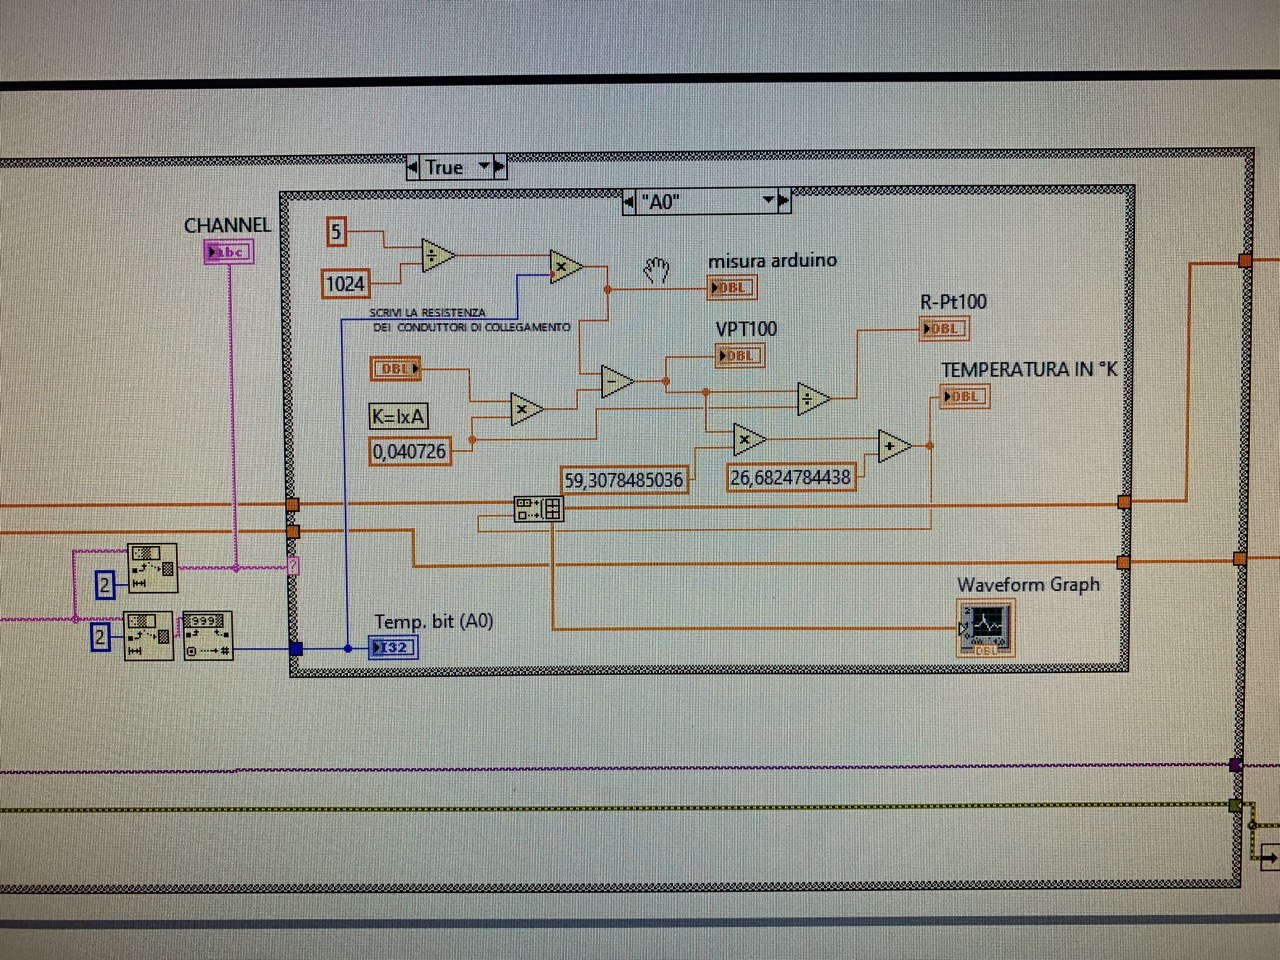
\includegraphics[width=0.9\textwidth]{../lessons/image/14/1.jpg}
\caption{\label{fig:14_1} Convertire voltaggio in temperatura con LabView.}
\end{figure}

\subsection{Tensione \(V_{out}\) (analog pin A1)}

Per quanto riguarda la misura della tensione in uscita \(V_{out}\) dall'amplificatore, viene semplicemente calcolato il valore in tensione. Lo schema in LabView è riportato in Fig. \ref{fig:14_2}.

\begin{figure}[h!]
\centering
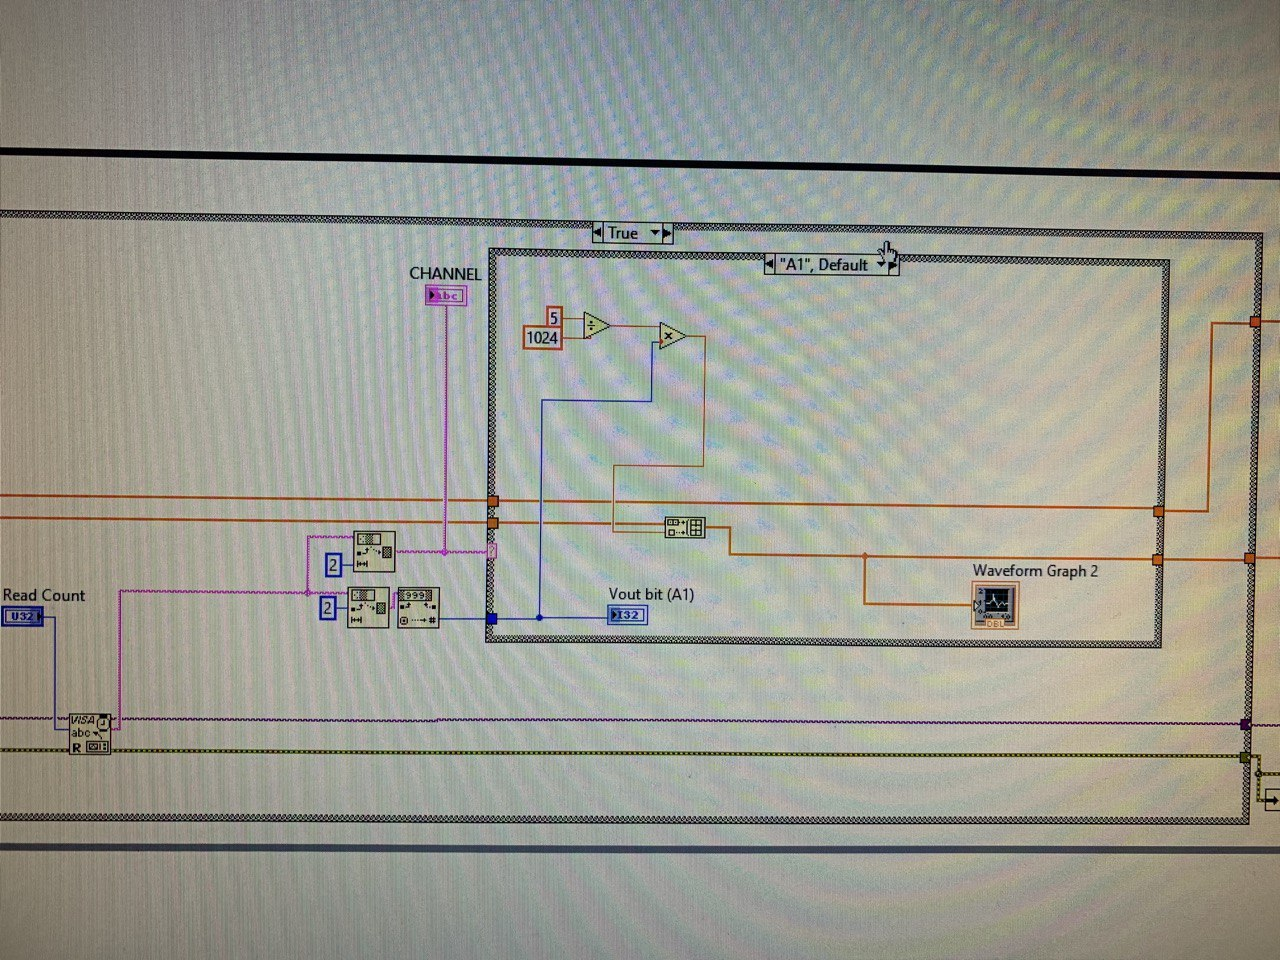
\includegraphics[width=0.9\textwidth]{../lessons/image/14/2.jpg}
\caption{\label{fig:14_2} Misurare voltaggio in LabView.}
\end{figure}

\section{Disaccoppiamento termico termometro e campione}
Nella prima parte di questa giornata abbiamo cercato di disaccoppiare termicamente il termometro sul campione e la camera. In particolare, nella giornata di ieri riuscivamo a raffreddare la camera fino a 66 K, mentre il termometro del campione rimaneva a circa 120 K.

Per sistemare questo problema, abbiamo riaperto il campione e tolto il rivestimento che lo faceva assomigliare ad una mummia. Abbiamo dunque tolto tutto e l'unica cosa che abbiamo inserito è un sottile strato di MAINLAR che riveste il superconduttore e i suoi contatti.

Abbiamo riattaccato il campione nella camera come precedentemente e abbiamo aggiunto una cupola di alluminio (un alluminio un po' più spesso di quello normale) per isolare il campione e il suo termometro da radiazioni.


\marginpar{ \textbf{Laboratory 15.} \\  \displaydate{date}. \\ Compiled:  \today.}

\section{Secondo test preliminare}

Una volta fatte le modifiche della prima parte, abbiamo ricollegato tutto. Un arduino è stato collegato al pt100 della camera per monitorarne la temperatura. Un altro arduino è stato collegato al potenziale di uscita dal circuito dell'amplificatore per vedere se osserviamo il salto dato dalla transizione del superconduttore.

Alla fine siamo riusciti a raffreddare la camera fino a 37 K (dopo circa 2 ore) e il termometro del superconduttore segnava circa 65 K. I progressi ottenuti dal disaccoppiamento sono dunque ottimi. Le misure effettuate sono riportate in Fig. \ref{fig:15_1}.

Il problema principale di tutto è che non siamo riusciti ad osservare il salto. Abbiamo notato che la tensione da 30 mV è salita fino ai 420 mV in modo lineare. Non osservando ancora il salto a temperature abbastanza basse (in cui ci aspettiamo che il campione abbia raggiunto effettivamente almeno una temperatura di 80 K), controlliamo che il circuito dell'amplificatore sia apposto. Il problema gravissimo è che cambiando la tensione in ingresso per esempio da 2.5 V a 1 V (o addirittura azzerandola!) il potenziale in uscita rimane costante a 420 mV! Abbiamo un problema gravissimo che dobbiamo assolutamente risolvere.

Per prima cosa abbiamo connesso una resistenza di 10 \( \Omega  \) al posto dei 4 fili del superconduttore. I valori ottenuti sembrano scalare linearmente cambiando il potenziale in ingresso. Però osserviamo che sono sempre più alti rispetto all'aspettazione teorica. Abbiamo azzerato il potenziale in ingresso: otteniamo circa 90 mV. A cosa sono dovuti? L'amplificatore non funziona più? Le altre volte avevamo ottenuto a 0 V in ingresso 0 V in uscita, com'è logico che sia. Dobbiamo risolvere questo problema.


\begin{figure}[h!]
\centering
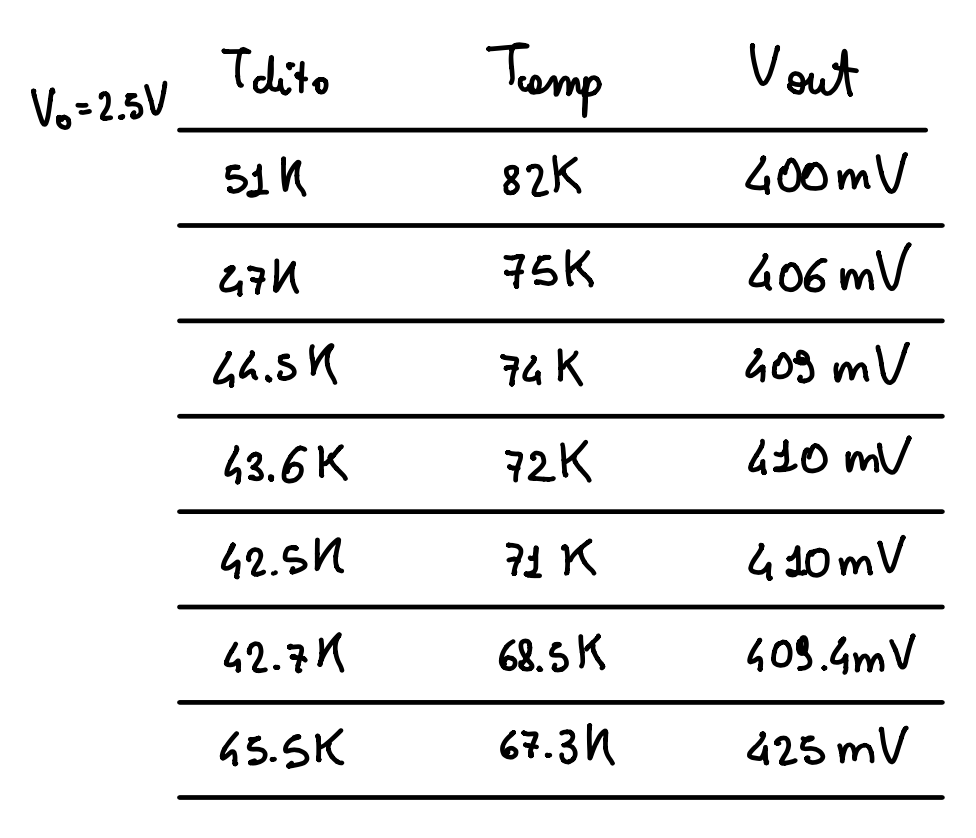
\includegraphics[width=0.7\textwidth]{../lessons/image/15/1.png}
\caption{\label{fig:15_1} Misure effettuate durante il raffreddamento.}
\end{figure}


\end{document}
